\section{MIBot System Design}
\label{sec:deployment}


\subsection{Overview of the Application}


MIBot is implemented as a containerized software system that can be run locally for development and deployed to cloud-based systems. In this section, we discuss the implementation details of MIBot, from the structure of the Python microservice and its integration with the OpenAI API to the containerization and the deployment of the service on Amazon Web Services.

At the heart of MIBot is a lightweight Python web application built with the \texttt{Sanic} framework \cite{pi_sanic}. In MIBot, \texttt{app.py} --- the main entry point --- uses \texttt{Sanic} to configure routes for all external interactions and instantiates the conversation engine.
\begin{figure}[ht]
  \centering
  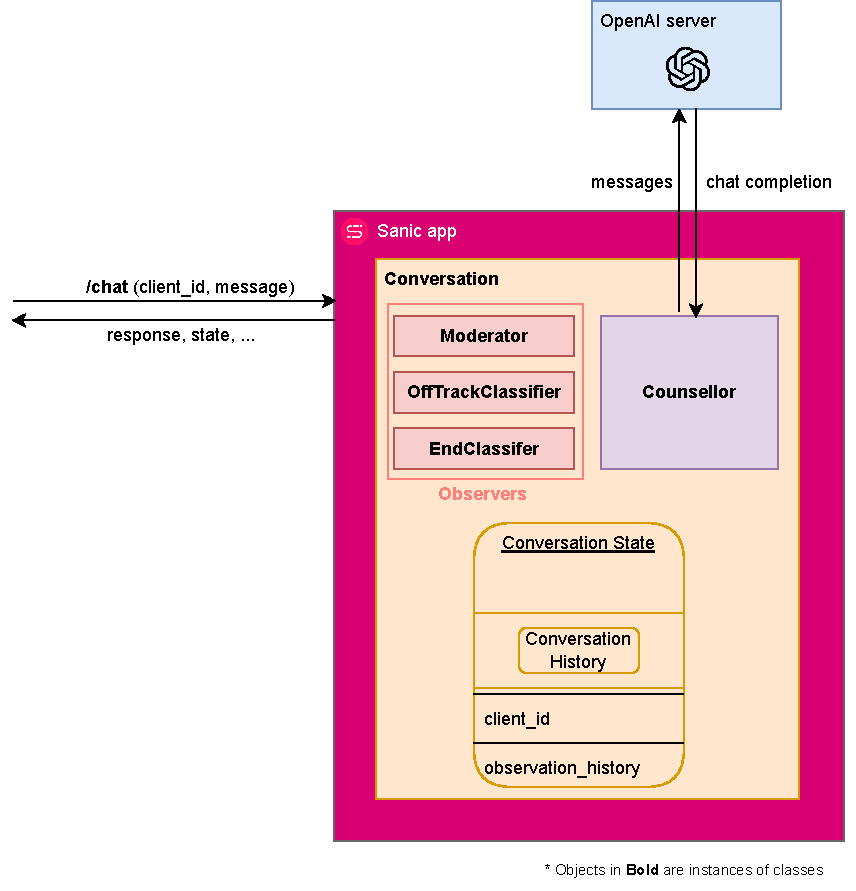
\includegraphics[width=0.7\linewidth]{fig/microservice.drawio.pdf} 
  \caption{Overview of the Sanic application that contains MIBot code and exposes REST APIs.}
  \label{fig:microservice}
\end{figure}
At the start of a conversation, the \texttt{Conversation} object is initialized, which creates and stores a list of \texttt{Observer} instances. It also creates a \texttt{Counsellor} object that encapsulates the chatbot logic (Figure~\ref{fig:microservice}). When a user sends a request to the \texttt{/chat} endpoint containing the client's message and \texttt{client\_id} in a structured JSON object, Sanic's route handler updates the state of the \texttt{Conversation} and requests the next turn from it. The \texttt{Conversation} object relays this to the \texttt{Counsellor}, which in turn sends a request to the OpenAI API with the accumulated conversation history and the current client message, and receives a \texttt{ChatCompletion} response. The \texttt{ChatCompletion} response contains the generated counsellor turn, which is returned to the \texttt{Conversation} object.

Each \texttt{Observer} attached to the \texttt{Conversation} inherits from a base class defining an asynchronous \texttt{observe()} method. As noted earlier, the \texttt{Moderation} observer screens counsellor utterances for safety and appropriateness; the \texttt{Offtrack} observer assesses whether the client is steering the conversation away from smoking cessation; and the \texttt{EndClassifier} determines when a session should conclude. These observers are implemented as separate GPT-4o API calls with their own prompts. After each turn, the \texttt{Conversation} object loops through all \texttt{Observer} objects, collects their observations, and makes real-time decisions (e.g., whether to end the conversation) before updating its state. If the generated output from the \texttt{Counsellor} is deemed suitable for the client, it is passed to Sanic's response handler, which packages it with metadata into a JSON object and sends it to the client.

A single \texttt{Sanic} app can handle multiple clients at once by creating replicas of the \texttt{Conversation} object, each uniquely identified by the \texttt{client\_id}.\footnote{For the human feasibility study, in order to keep track of the participants and their conversations, we explicitly use \texttt{prolific\_id} as \texttt{client\_id}. Prolific (\url{www.prolific.com}) is the platform we use to recruit participants and conduct our feasibility study. See Section~\ref{sec:feasibility-study} for further details.} The microservice also exposes some additional endpoints: \texttt{/get\_transcript} provides a downloadable transcript of the conversation for post-session analysis; \texttt{/health} returns a simple \texttt{200} response so that load balancers and orchestrators can perform health checks; and \texttt{/info} exposes build metadata such as the current version of the prompt.

\subsection{Containerization}

\begin{figure}[ht]
  \centering
  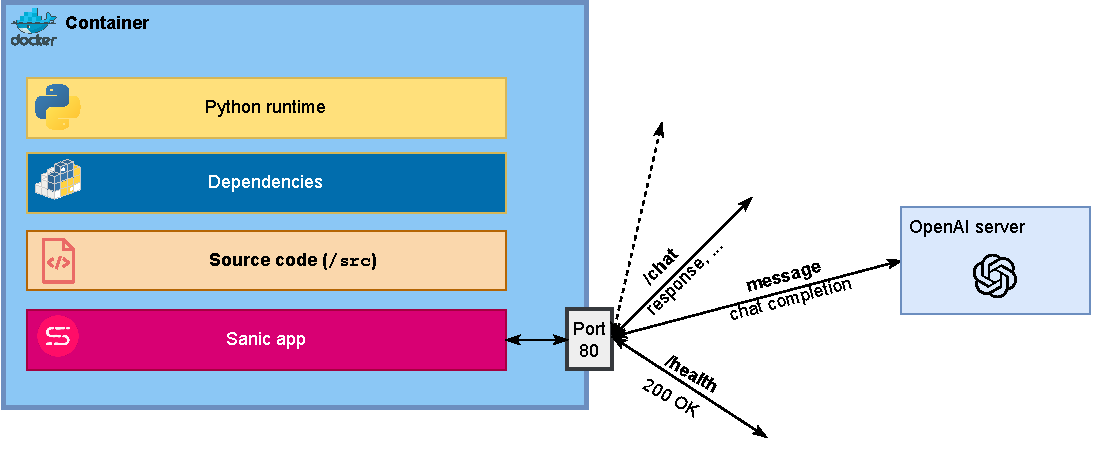
\includegraphics[width=0.7\linewidth]{fig/container.drawio.pdf} 
  \caption{Containerized Sanic application.}
  \label{fig:containerization}
\end{figure}

For reproducibility and ease of deployment, the microservice is packaged in a Docker container. Containerization provides several advantages for the development, testing, and deployment of MIBot:

\begin{itemize}
\item \textbf{Environment Consistency:} Containers encapsulate all dependencies, ensuring that the application behaves identically across local development machines, staging environments, and production servers. This eliminates the ``works on my machine'' problem.

\item \textbf{Portability:} The same container image can run on any system that supports Docker (or an OCI-compliant runtime), whether on a developer's laptop, an on-prem cluster, or a cloud provider like AWS, without modification.

\item \textbf{Isolation:} The application runs in its own isolated environment with a defined set of libraries and runtime parameters, preventing conflicts with other software on the host system.

\item \textbf{Scalability:} Container orchestration platforms such as Kubernetes or Amazon ECS can rapidly start and stop containers based on demand, enabling efficient horizontal scaling during high-traffic periods.

\item \textbf{Faster Deployment and Rollback:} Pre-built container \emph{images} can be deployed quickly, and previous versions can be rolled back by redeploying an earlier image tag, reducing downtime.

\item \textbf{Simplified CI/CD Integration:} Containers integrate seamlessly with continuous integration and delivery pipelines, allowing automated builds, tests, and deployments triggered by code changes.

\item \textbf{Reproducibility:} For experimental settings, distributing a container image ensures that collaborators can reproduce results exactly, regardless of local environment differences.
\end{itemize}

The MIBot container image is defined by a \texttt{Dockerfile} specifying the base Python runtime, required dependencies, the source code, and main entry point (\emph{viz.} \texttt{app.py}). This image is stored in Amazon Elastic Container Registry (ECR). The container registry stores all the images built by the CI/CD pipeline, but only the image with the \texttt{production} tag is used for deployment.

\section{Deploying MIBot to AWS}
\label{sec:mibot-deployment}

MIBot is deployed as a service on Amazon \textbf{Elastic Container Service (ECS)}. ECS is a fully managed service provided by Amazon Web Services (AWS) that ``simplifies the deployment, management, and scaling of applications using containers'' \cite{aws-ecs-getting-started}. We now discuss each component of ECS.

\subsection{Components of ECS}
\begin{figure}[ht]
  \centering
  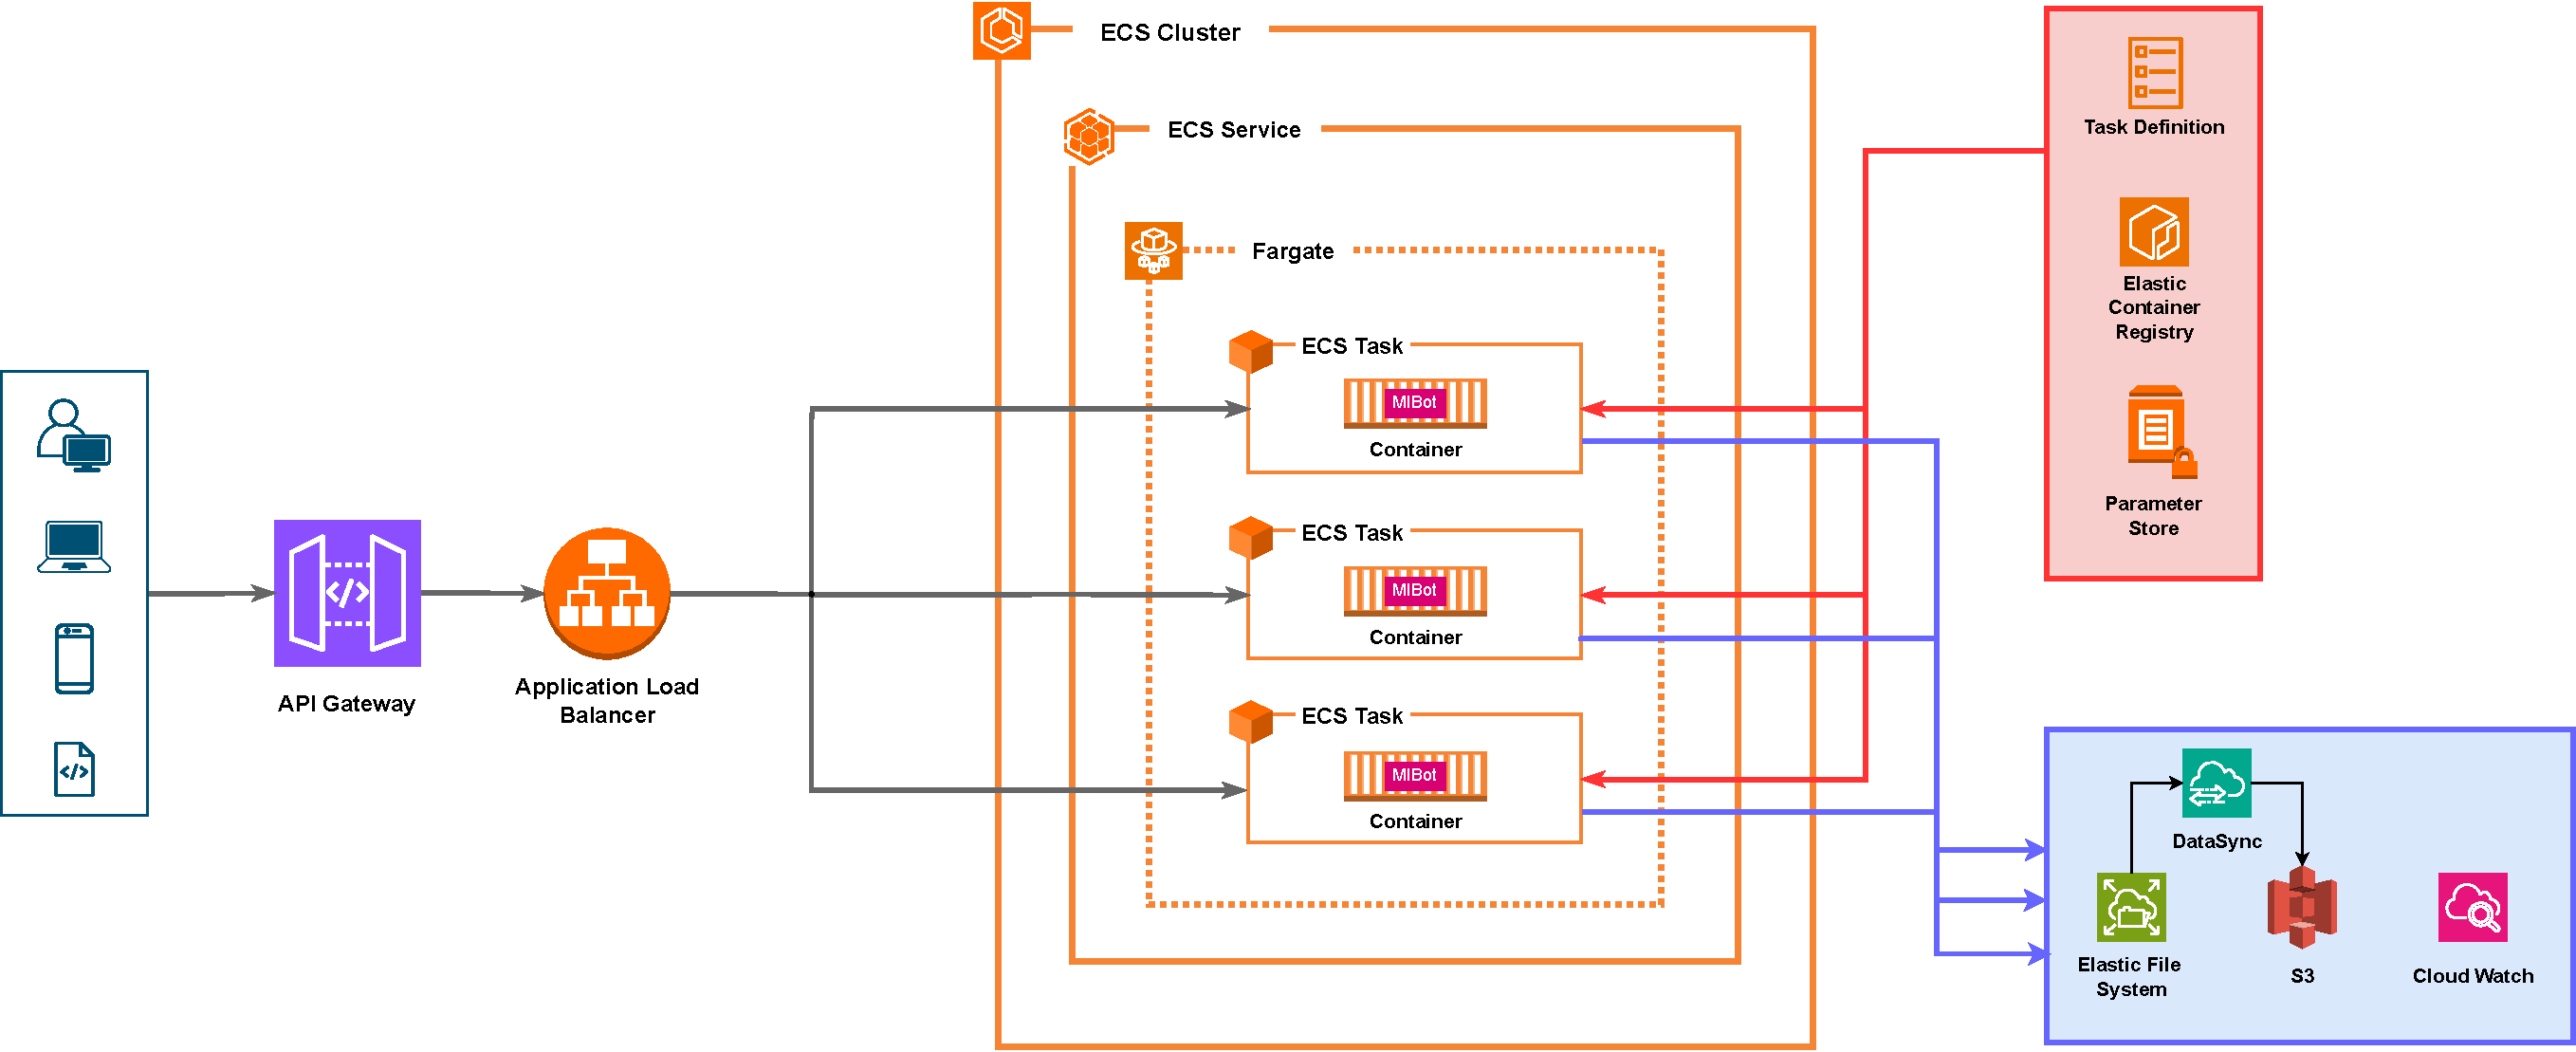
\includegraphics[width=0.99\linewidth]{fig/deployment.drawio.pdf} 
  \caption{Containerized MIBot application deployed to ECS.}
  \label{fig:ecs-components}
\end{figure}

\paragraph{1. ECS Cluster:}To deploy MIBot to ECS, we first provisioned an \textbf{ECS cluster} (\texttt{mibot-v6-cluster}). An ECS cluster is a \textit{logical} grouping of heterogeneous compute resources. To understand what we mean by this, let's first see what a compute resource is in the context of AWS. An AWS \textbf{compute resource} is any AWS-managed infrastructure component that provides processing power for running applications or workloads. Examples include Elastic Cloud Compute (EC2), AWS Lambda, AWS Fargate, etc. Some of the compute resources are \textbf{user-managed}, like EC2, where users rent virtual machines to run and manage their applications. In contrast, AWS Fargate is \textbf{fully managed} and is used to run containerized applications. A cluster is merely a logical grouping of such compute resources.

In our ECS cluster, however, we only used \textbf{AWS Fargate} as the computing resource. Apart from the ability to deploy the containerized MIBot application without having to manage our own servers, AWS Fargate also provided us with \emph{spot runs} for cost optimization. In the \texttt{FARGATE\_SPOT} mode, tasks run on spare compute capacity. If a container receives no traffic in the last two hours and AWS needs the capacity back, the task will be terminated. ECS will detect this event and will almost immediately instantiate a new task for the application.

\paragraph{2. ECS Service:}Inside the ECS cluster, we created an \textbf{ECS Service} (\texttt{mibot-v6-service}). The ECS Service contains the deployment configuration of the application. For example, the number of desired replicas of the application (also called \emph{tasks}) that should run at any given time.  For our study, we set this to use two tasks. If one of the tasks fails for some reason, the ECS Service replaces it automatically. It can also be configured to increase the number of tasks when it detects higher-than-normal traffic. The Service is connected to an Elastic Load Balancer (ELB) to distribute incoming traffic evenly among tasks. Most importantly, it also defines deployment (rolling update, blue/green deployment) and rollback strategies. It can leverage the AWS circuit breaker to roll back failed deployments automatically.

\paragraph{3. ECS Task Definition:}The final piece in MIBot's deployment is defining a \textbf{Task}. A \texttt{Task} runs a specific container after downloading it from the Elastic Container Registry (ECR). The \texttt{Task} definition specifies environment variables and API credentials that are securely stored in AWS Systems Manager Parameter Store and are injected into the container (e.g., \texttt{OPENAI\_API\_KEY}) when the task is started. It further defines a \emph{health check} for the container. The health check sends a request to the \texttt{/health} endpoint on the container's port~80 every five minutes. If the response is anything other than \texttt{OK 200} or it does not get a response within one minute, it deems the container unhealthy. The \texttt{Service} terminates the \texttt{Task} and replaces it with a new one. The task definition further contains required CPU and memory (1024 mcpu and 4~GB, respectively, in the case of MIBot). The containers also mount a persistent Amazon Elastic File System (EFS) volume to store conversation transcripts and evaluation metrics. Furthermore, all container logs are written in AWS CloudWatch for retrospective analysis of the system's behaviour.

\subsection{Other Components of the Deployment}

\paragraph{Load Balancer:}We configured an Elastic Load Balancer (\texttt{mibot-elb}) with three subnets for high availability, meaning we have three instances of load balancers in three different Availability Zones. The load balancers are the modern \emph{application} load balancers (ALB), which are internet-facing and associated with a security group permitting inbound traffic on port 443. The DNS names allow external users to connect to the service through a friendly domain. The ALB routes incoming HTTP requests to the ECS service's target group and internal health check requests to the \texttt{/health} endpoint.

\paragraph{API Gateway:}We also provisioned an AWS API Gateway, which acts as a reverse proxy and enables secure TLS termination and request throttling. The gateway exposes HTTPS endpoints for \texttt{/chat}, \texttt{/get\_transcript}, \texttt{/health}, \texttt{/info}, and \texttt{/s3\_upload}. Each path includes \texttt{OPTIONS} methods to enable cross-origin requests and defines the expected response headers. This allows client browsers (running the frontend code) to send requests to MIBot without getting a ``Cross-Origin Request Blocked'' error or ``Not Secure'' warning.

\paragraph{DataSync:}Conversation transcripts and metadata are stored on both an encrypted EFS volume and AWS S3 only when the participant clicks on the final Submit button at the end of the study session. EFS acts as a redundant data layer in case the upload to S3 fails for some reason. For eventual consistency, we periodically copy files from EFS to S3 with the help of AWS DataSync, which runs a daily CRON job.

\subsection{Deployment Pipeline}
We adopted automated development practices for deployment. Every time we push a special `\texttt{production}' Git tag to the remote main branch, a GitHub Workflow builds the Docker image, runs unit tests, and, if tests pass, pushes the image to Amazon ECR. Another workflow triggers a CloudFormation deployment that updates the ECS task definition with the new image tag and performs a rolling deployment of the ECS Service. Deployment uses a circuit breaker configuration: if the service fails health checks, the rollout is automatically rolled back to the previous stable revision. By integrating the deployment pipeline into version control, we ensured automated deployments tied to code changes.
